\section{The Bayesian feedback loop on the OPX}
\label{sec:feedback}

\statusbox{Status of this port.}{Implemented, speed pass ``3b'' (2026-09-25):
\file{kexp/experiments/opx\_sequences/feedback.py} (\code{make\_feedback\_sequence},
\code{feedback\_constants}, \code{build\_feedback\_shot\_tables},
\code{\_feedback\_body}, \code{feedback\_finish} and the table helpers),
\file{HF\_experiments/feedback/\{expt\_params\_feedback\_opx, feedback\_opx,
feedback\_opx\_deterministic\}.py}, \file{kexp/analysis/feedback\_opx.py}
(\code{FeedbackOPXReplay}, \code{posterior\_update\_fixed\_point\_emulation},
\code{run\_shot\_fixed\_point\_emulation}, \code{true\_bloch\_step}), the
additive host helpers at the end of \file{kexp/base/feedback.py}, and
\file{tests/test\_feedback\_opx.py} (28 items). Offline-tested against the
double-precision ARTIQ posterior; compiled and timed on the QOP simulator
through \code{OPXBench} (section~\ref{sec:feedback:speed}). \textbf{Not run
on hardware.} Every calibration constant it uses was measured through the
ARTIQ path and is a placeholder until re-taken in OPX units
(section~\ref{sec:feedback:calib}). The remesh is a design only
(section~\ref{sec:feedback:remesh}).}

\subsection{The physics in plain words}

Per shot, ARTIQ prepares one spin-polarised ensemble in the HF tweezer
(state $|1,-1\rangle$, Bloch vector $z = +1$) and hands the atoms to the OPX.
The OPX then runs $N$ cycles ($N = $ \code{N\_pulses}: 17 in
\code{feedback\_opx.py}, 9 in the open-loop sweep) of:

\begin{enumerate}[nosep]
  \item a Raman pulse of pre-drawn random duration $\tau_i \in [0.5, 1.0]\,t_\pi$
    (uniform, a pure function of the shot's seed, rounded to the 4\nsu\ clock)
    at the current drive frequency, rotating the Bloch vector about an axis
    that depends on how far the drive is from the true two-photon resonance
    $\omega_0$ (\code{frequency\_raman\_transition} $= 119.4639$\,MHz, $t_\pi =
    7.121\us$, $\Omega/2\pi = 1/(2t_\pi) = 70.2$\,kHz);\footnote{\file{kexp/config/expt\_params.py}
    lines 166, 373.}
  \item a 5\us\ imaging pulse at the ``midpoint'' detuning
    (\code{frequency\_detuned\_hf\_midpoint} $= -519.5$\,MHz), whose dispersive
    signal integrated on the APD is a \emph{weak measurement} of $S_z$: expected
    photon fraction $p_1(z) = \tfrac12(1+z) + (m_f - \tfrac12)(1 - z^2)$,
    $m_f = 0.4719$, which maps $z \in [-1, 1]$ monotonically onto $[0, 1]$
    for any $m_f \in (0.25, 0.75)$; the light also AC-Stark-shifts the levels
    by $f_{LS} = 40.61$\,kHz, a $z$-rotation of $\phi_{LS} = f_{LS}\,t_{\rm img} =
    0.203$ turns per measurement, and scatters photons that shrink the
    transverse spin by $C = 0.62$ (\code{back\_action\_coherence}); $z$ is not
    touched by the measurement;\footnote{\file{HF\_experiments/feedback/expt\_params\_feedback.py}
    lines 43--69; the coherence was fitted with the light shift pinned, and
    the pair is not a self-consistent joint fit (``residuals are still 83x
    the APD error bars'').}
  \item a Bayesian update: for each of $m = 21$ hypotheses $\omega_j$ on a grid
    of $\pm\,$\code{feedback\_guess\_span\_Omega}$\,\Omega$ around the nominal
    resonance plus an integer offset (span 3, offset 2 in \code{feedback\_opx.py}:
    step $0.3\,\Omega = 21$\,kHz), snapped so one point sits exactly on the
    nominal resonance (index \code{zidx}), propagate a Bloch vector through
    the pulse and the measurement, weight it by the Gaussian likelihood of
    the observed photon fraction with the \emph{fixed} detector width
    $\sigma_p = \sigma_n / n = 212.75 / 1336.2 = 0.159$, and drive the next
    pulse at the \textbf{posterior argmax grid point}. The first pulse is
    driven at the grid point nearest \code{feedback\_fractional\_initial\_offset}.
\end{enumerate}

The multi-pulse frequency sensitivity is Ramsey-like: what distinguishes
hypotheses is the phase each accumulates between pulses relative to the
drive. Hence the drive phase at every pulse start must be known.

\subsection{The reset phase model and its consequence (D4)}
\label{sec:feedback:phase}

On ARTIQ the AD9910s run phase-continuous: the physical two-photon drive
phase is the integral of the programmed frequency, and
\code{RamanBeamPair.io\_update\_and\_phase\_update} reconstructs it in integer
FTW arithmetic. The posterior then uses $\phi_{j,i} = \phi_{\rm drive}(t_i) -
\omega_j t_i$. On the OPX the IF phase is a function of absolute time and the
current frequency; instead of rebuilding a tracker, the port uses the
\textbf{reset model}, selected by the integer parameter
\code{feedback\_phase\_model\_reset = 1} (the sequence refuses any other
value):

\begin{quote}
Both Raman analog drives get \code{reset\_if\_phase}, applied by an
\code{align(raman\_80, raman\_150, raman\_switch)} immediately before every
pulse's \code{play('pass', 'raman\_switch', duration=}$\tau_i$\code{)}, so the
two-photon drive phase at every pulse start is 0 (plus a hardware constant
common to all pulses). The posterior uses $\phi_{\rm drive} = 0$ and the
hypothesis term $\phi_{j,i} = -f_j t_i \pmod 1$ (turns), $t_i$ the start of
pulse $i$ from the start of pulse 0. No phase tracker runs on the OPX.
\end{quote}

A constant common phase offset is harmless: the initial state is on the
pole, the measurement is $S_z$, and every operation in the model commutes
with a global $z$-rotation. In the frame rotating at hypothesis $j$ the state
is \emph{static} between pulses: only the pulse \emph{starts} enter the model
(through the azimuth of the rotation axis), and the light-shift and
drive-frame $z$-rotations commute with the free precession. The gaps between
a pulse's end and the exposure, or between the exposure and the next pulse,
do not enter at all -- what must be exact is $t_i$.

\paragraph{The consequence.} With a per-pulse reset, the phase the atoms
accumulate relative to the drive between pulses is $\omega_0\,\Delta t$, not
$(\omega_{\rm drive} - \omega_0)\,\Delta t$:
\[
  f_0 \times 4\nsu = 119.4639\,\mathrm{MHz} \times 4\nsu = 0.478\ \text{turns per clock cycle}.
\]
One cycle of unplanned delay anywhere in the loop rotates every hypothesis
axis by almost half a turn; on ARTIQ the same error costs $\Delta\omega\,\delta
t \sim 10^{-3}$ turns. The reset model trades the tracker for \textbf{exact
knowledge of the pulse-start times in clock cycles}. Three things make that
true:

\begin{enumerate}[nosep]
  \item Every per-step interval is computed on the host from the drawn
    pulse-time list (section~\ref{sec:feedback:schedule}), and the OPX is held
    to it by a per-step wait on the Raman switch element. The Raman play is
    emitted with \code{min\_cc} (the run's shortest drawn duration), so no
    per-shot \code{if\_} guard -- which would add an implicit align and
    non-deterministic cycles -- sits in front of it; the tables refuse a draw
    that rounds below 4\,cc.
  \item The \emph{actual} start of every pulse is recorded with one timestamp
    stream, \code{t\_pulse\_start\_cc} (the Raman \code{'pass'} play) -- the
    only timestamp the model needs. The replay uses the actual times by
    default; the finish hook recomputes the schedule from the saved durations
    and the params and prints a \code{***} line with the largest
    scheduled-vs-actual deviation if any pulse is off it.
  \item The real-time loop uses the \emph{scheduled} times: the host
    precomputes the hypothesis-frame tables from the schedule and ships them
    per shot, so the OPX computes no phase at all.
\end{enumerate}

\subsection{The per-step schedule}
\label{sec:feedback:schedule}

We write $\tau_i$ for the drawn duration of pulse $i$ (the code's
\code{d\_cc[i]}; the code's \code{d} is the \emph{drive index}, below). Per
pulse, in program order, as \code{\_feedback\_body} emits
it:\footnote{\file{kexp/experiments/opx\_sequences/feedback.py},
\code{\_feedback\_body}; the statement list is in its module docstring.}

\begin{lstlisting}[style=py]
[assign(d, sched_arr.at(i))]                            # open loop only: drive index of pulse i
assign(if80, if80T[d]); assign(if150, if150T[d])        # the grid point's two integer IFs (Hz)
ctx.set_frequency('raman', if80, which='raman_80')      # update_frequency on each drive
ctx.set_frequency('raman', if150, which='raman_150')
ctx.raman_pulse(d_arr.at(i), phase_reset=True,          # reset_if_phase x2, align(drives, switch),
                timestamp_key='t_pulse_start_cc',       #   pass tau_i (timestamped), block
                min_cc=min_d_cc)                        #   -- no if_ guard
ctx.align('raman', 'imaging')                           # the exposure follows the pulse
v = ctx.measure('apd', role='imaging', expose=True,     # align(imaging_switch, apd); pass t_img;
                t_expose=c.t_img_s)                     #   block; ADC window; save(v)
ctx.wait_cc(wait_arr.at(i), 'raman')                    # the per-step hold, raman_switch only
<p_meas, per-pulse seeds, one loop over j, argmax>       # the update: runs inside the hold
ctx.save('drive_index', d); ctx.save('s_z', z[zidx])
with ctx.for_range(m) as j: ctx.save('log_weights', L[j] - M)
[assign(d, jmax)]                                       # closed loop only: next drive
\end{lstlisting}

On \code{raman\_switch} the statements per pulse are exactly: align (the
phase reset lands here), pass $\tau_i$, block ($E = 4$\,cc), align with
\code{imaging\_switch}, wait -- and nothing else (asserted by
\code{test\_sequence\_traces\_offline} on the op log). The imaging exposure
runs on \code{imaging\_switch} and the ADC window on \code{apd}. The per-step
interval and the hold are

\begin{align*}
  \mathrm{gap}_i &= \tau_i + E + t_{\rm img} + E + B + O + X, \qquad t_0 = 0,\quad t_{i+1} = t_i + \mathrm{gap}_i,\\
  \mathrm{wait}_i &= \mathrm{gap}_i - \tau_i - E - O = t_{\rm img} + E + B + X \quad (\text{cycles}),
\end{align*}
with $t_{\rm img} = 1250$, $B$ = \code{s\_to\_cc(t\_opx\_feedback\_compute\_budget)}
$= 2500$, $O$ = \code{t\_opx\_feedback\_align\_overhead} (328\nsu) $= 82$ (86 with
discrete durations, \code{t\_opx\_feedback\_align\_overhead\_levels}), the constant
sync cost of the aligns and the frequency update, and $X$ =
\code{t\_feedback\_extra\_gap} $= 0$, a free knob like ARTIQ's
\code{delta\_t\_mu}. This is ARTIQ's \code{compute\_t\_between\_pulses\_mu}
per step (\code{feedback\_step\_gaps\_cc}; the cumulative sum is
\code{schedule\_pulse\_starts} in \file{kexp/base/feedback.py});
\code{wait}$_i$ is shipped as an int shot array indexed by the pulse
counter. Why the hold contains $t_{\rm img} + E$: the align does not stall
the Raman switch (\code{imaging\_switch} is idle when it is reached), so the
hold starts right after the Raman block and the exposure runs
\emph{concurrently} with its first $t_{\rm img} + E$ cycles; on the simulator a
hold of $B + X$ alone made every interval exactly $t_{\rm img} + E$ short.
The update is issued after the measure statement, and \code{measure} blocks
the program thread until the ADC result exists, so the update cannot overlap
the exposure and $B$ must cover the whole of it.

\begin{figure}[htbp]
\centering
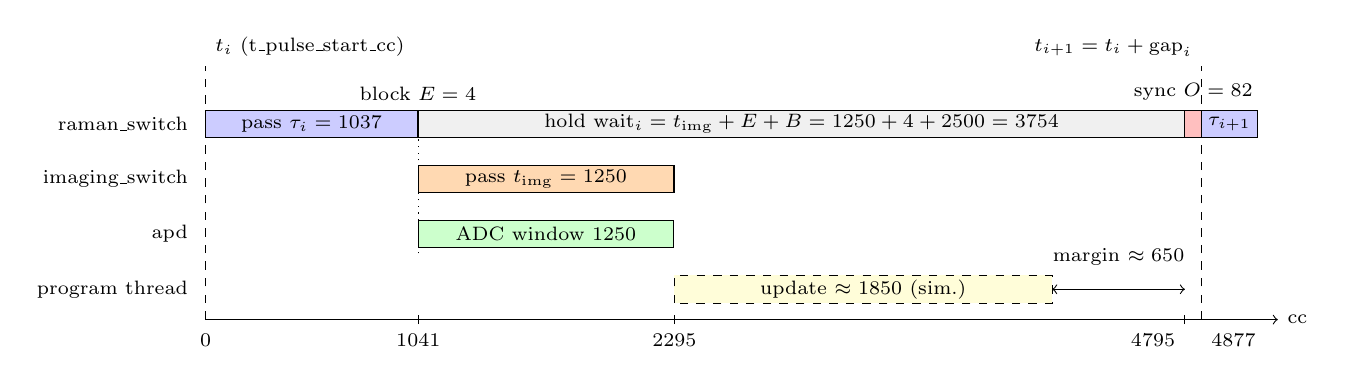
\begin{tikzpicture}[x=0.0026cm, y=0.7cm, font=\scriptsize]
  % row labels
  \node[anchor=east] at (-40,3.25) {\code{raman\_switch}};
  \node[anchor=east] at (-40,2.25) {\code{imaging\_switch}};
  \node[anchor=east] at (-40,1.25) {\code{apd}};
  \node[anchor=east] at (-40,0.25) {program thread};
  % pulse starts
  \draw[dashed] (0,-0.3) -- (0,4.3);
  \draw[dashed] (4877,-0.3) -- (4877,4.3);
  \node[anchor=south west] at (0,4.3) {$t_i$ (\code{t\_pulse\_start\_cc})};
  \node[anchor=south east] at (4877,4.3) {$t_{i+1} = t_i + \mathrm{gap}_i$};
  % raman_switch
  \draw[fill=blue!20] (0,3.0) rectangle (1037,3.5);
  \node at (518,3.25) {pass $\tau_i = 1037$};
  \draw[fill=black] (1037,3.0) rectangle (1041,3.5);
  \node[anchor=south] at (1039,3.5) {block $E = 4$};
  \draw[fill=gray!12] (1041,3.0) rectangle (4795,3.5);
  \node at (2918,3.25) {hold $\mathrm{wait}_i = t_{\rm img} + E + B = 1250 + 4 + 2500 = 3754$};
  \draw[fill=red!25] (4795,3.0) rectangle (4877,3.5);
  \node[anchor=south] at (4836,3.5) {sync $O = 82$};
  \draw[fill=blue!20] (4877,3.0) rectangle (5150,3.5);
  \node at (5013,3.25) {$\tau_{i+1}$};
  % imaging_switch
  \draw[dotted] (1041,0.9) -- (1041,3.0);
  \draw[fill=orange!30] (1041,2.0) rectangle (2291,2.5);
  \node at (1666,2.25) {pass $t_{\rm img} = 1250$};
  \draw[fill=black] (2291,2.0) rectangle (2295,2.5);
  % apd
  \draw[fill=green!20] (1041,1.0) rectangle (2291,1.5);
  \node at (1666,1.25) {ADC window 1250};
  % program thread
  \draw[dashed, fill=yellow!15] (2295,0.0) rectangle (4145,0.5);
  \node at (3220,0.25) {update $\approx 1850$ (sim.)};
  \draw[<->] (4145,0.25) -- (4795,0.25);
  \node[anchor=south] at (4470,0.5) {margin $\approx 650$};
  % axis
  \draw[->] (0,-0.3) -- (5250,-0.3);
  \node[anchor=west] at (5250,-0.3) {cc};
  \draw (1041,-0.38) -- (1041,-0.22);
  \draw (2295,-0.38) -- (2295,-0.22);
  \draw (4795,-0.38) -- (4795,-0.22);
  \node[anchor=north] at (0,-0.38) {0};
  \node[anchor=north] at (1041,-0.38) {1041};
  \node[anchor=north] at (2295,-0.38) {2295};
  \node[anchor=north east] at (4795,-0.38) {4795};
  \node[anchor=north west] at (4877,-0.38) {4877};
\end{tikzpicture}
\caption{One feedback cycle as scheduled, in 4\nsu\ clock cycles, for the
first drawn pulse of the simulated shot ($\tau_0 = 1037$\,cc $= 4.15\us$) and
the default parameters ($t_{\rm img} = 1250$, $B = 2500$, $O = 82$, $X = 0$):
$\mathrm{gap}_i = \tau_i + 3840$\,cc. The exposure and the ADC window are drawn
starting at the Raman block's end; the aligns delay them by a few cycles (in
the first-pass structure the exposure started 9\,cc after the Raman pass
ended: the 4-cc block plus 5\,cc of sync), inside the hold, without moving
$t_{i+1}$. The program-thread row is the simulator's per-pulse compute for the
default structure (1938\,cc including the 82-cc sync,
section~\ref{sec:feedback:speed}), placed after the exposure; it is a
measured duration, not a timestamp. The next pulse's IF update, phase reset
and align are the sync $O$.}
\label{fig:feedback:cycle}
\end{figure}

With the default numbers a cycle is $\tau_i + 3840$\,cc $= 18.9$--$22.5\us$
for $\tau_i = 890$--$1780$\,cc ($0.5$--$1.0\,t_\pi$), against ARTIQ's
57--61\us\ (section~\ref{sec:why}).

\paragraph{Why the overhead must be exact.} The OPX's real-time posterior
uses the \emph{scheduled} starts: the frame advance of hypothesis $j$ over
step $i$ is $\operatorname{frac}(f_j\,\mathrm{gap}_i)$
(section~\ref{sec:feedback:numerics}). If the true constant $O$ differs from
the parameter by one cycle, every hypothesis's phase is wrong by 0.478 turns
per step, and the error accumulates. The simulator shows it: with the
previous structure's value (91\,cc) on the pass-3b loop, the pulse starts
drifted by $-9$\,cc per interval ($0, -9, -18, \dots, -45$ over six pulses),
i.e.\ $9 \times 0.478 = 4.3$ turns per step; with 82\,cc (and 86\,cc for the
discrete-duration structure) the simulated slip is 0 on every pulse. The
replay, which uses the timestamps, is unaffected either way.

\subsection{The exact applied frequency}
\label{sec:feedback:freq}

The drive of every pulse is a \emph{grid index} $d$: the control law picks the
argmax, and the initial drive is snapped to the grid point nearest
\code{feedback\_fractional\_initial\_offset} (the grid is built around the
rounded offset, so with the default grid -- offset 0, span 5 -- the snap is
the identity; with the \code{feedback\_opx.py} config -- offset 2, span 3 --
the grid snap onto resonance moves it $2.0 \to 2.1$, at most half a step in
general). For every grid point the host computes the two integer IFs once per
run from the Raman split,
\[
  \mathrm{IF}_{el}[j] = \mathrm{IF0}_{el} + \operatorname{round}\big(s_{el}\, w_j\, f_\Omega\big),\qquad
  s_{80} = -\tfrac{8}{46},\quad s_{150} = +\tfrac{15}{46},\quad f_\Omega = \frac{1}{2t_\pi},
\]
with \code{IF0} and the slopes from \code{ctx.transition\_offset\_terms('raman')}
(the \code{RamanBeamPair} split, numerically differentiated at trace time), and
the OPX applies \code{if80T[d]}, \code{if150T[d]} with
\code{ctx.set\_frequency(..., which=)}. The two-photon frequency the atoms see
is, for the $+1/{+1}$ double-pass pair,
\[
  f_{\rm applied}[d] = 2\,\big(\mathrm{IF}_{150}[d] - \mathrm{IF}_{80}[d]\big),
\]
asserted at trace time to reproduce \code{frequency\_raman\_transition} from
the \code{IF0}s within 3\,Hz (and $2(s_{150} - s_{80}) = 1$ to $10^{-9}$). The
sequence streams $d$ per pulse (\code{drive\_index}) and records the integer
table (\code{if\_table\_hz}, shape $(m, 2)$), so the finish hook and the replay
know the applied frequency \emph{exactly}; every grid point is within 3\,Hz
($4\times 10^{-5}\,\Omega$) of $f_0 + w_j f_\Omega$
(\code{test\_if\_tables\_invert\_to\_the\_two\_photon\_frequency}). The QM
documentation gives no finite NCO quantum (``sub-Hz resolution'';
\code{update\_frequency} takes integer Hz ``in steps of 1''), so the integer
Hz commanded is taken as the applied frequency.

\subsection{The per-pulse algorithm on the OPX}
\label{sec:feedback:numerics}

QUA \code{fixed} is 4.28: range $[-8, 8)$, wrap modulo 16, and the
\code{Math} library has domain limits. Everything is therefore rescaled.
Frequencies are in units of $\Omega = \pi/t_\pi$, $w = (\omega - \omega_0)/\Omega$;
the grid is descending, $w_j = w_0 - j\,\Delta w$ ($\Delta w = 2\,\mathrm{span}/(m-1)$:
0.3 for span 3, 0.5 for span 5), with $w_{\rm zidx} = 0$ exactly. Rotation
angles are in turns.

\paragraph{Axis geometry from tables (idea A).} With the drive at index $d$,
the drive--hypothesis detuning is $\delta_j = w_d - w_j = (j - d)\,\Delta w$ and
depends only on $k = j - d \in [-(m-1), m-1]$. Five run tables of length
$2m - 1 = 41$, indexed by $j + (m - 1 - d)$, replace the per-point
\code{Math.inv\_sqrt}:
\[
  h_k = \sqrt{\tfrac{1}{16} + \big(\tfrac{k\,\Delta w}{4}\big)^2} = \frac{|H_k|}{4\Omega},\qquad
  u_{x,k} = \frac{\Omega}{|H_k|} = \frac{1}{4h_k},\qquad
  u_{z,k} = \frac{\delta}{|H_k|} = \frac{k\,\Delta w/4}{h_k},
\]
plus $u_{x,k}^2$ and $u_{x,k}u_{z,k}$. The tables refuse $(m-1)\Delta w > 10.9$
(so $h^2 < 8$).

\paragraph{Rotation angle and the sine table.} With $a_i = (\tau_i -
t_{\rm off})/(2t_\pi)$ (shipped as $-4a_i$, \code{theta\_scale\_x4}), the pulse
angle is $\theta_{i,k} = -4a_i\,h_k$ turns (the model's $-|H|\,\tau_{\rm ideal}$).
Its cosine and sine come from a table $T[n] = \sin(2\pi n/N)$, $N = 2^{12}$,
$n = 0, \dots, N + N/4 + 1$ (5122 entries), read from the 4.28 bit pattern
$u$ of $\theta$: $r = u \bmod 2^{28}$ (the fraction of a turn; negative angles
wrap correctly), $n = \lfloor r/2^{16}\rfloor$, $\varphi = (r \bmod 2^{16})/2^{16}$,
\[
  \sin 2\pi\theta \approx T[n] + \varphi\,(T[n+1] - T[n]),\qquad
  \cos 2\pi\theta \approx T[n + \tfrac N4] + \varphi\,(T[n + \tfrac N4 + 1] - T[n + \tfrac N4]),
\]
error $\le (2\pi/N)^2/8 = 2.9\times 10^{-7}$ on the trig values
(\code{opx\_sincos\_lut\_bits = 12}; 0 selects \code{Math.cos2pi}/\code{sin2pi}, exact).

\paragraph{Co-rotating azimuth frame with one merged $z$-rotation (idea D).}
The rotation axis of hypothesis $j$ at pulse $i$ is $\hat u = R_z(\phi_{j,i})\,\hat
u_0$ with $\hat u_0 = (u_x, 0, u_z)$, so $R(\hat u, \theta) = R_z(\phi)\,R(\hat u_0,
\theta)\,R_z(-\phi)$. The OPX keeps each hypothesis in the frame where its
next axis lies in the $x$--$z$ plane, $\tilde s_{j,i} = R_z(-\phi_{j,i})\,s_{j,i}$.
Then, with $c = \cos 2\pi\theta$, $s = \sin 2\pi\theta$ and $u_y = 0$, the Rodrigues
rotation has five distinct entries,
\[
  R(\hat u_0, \theta) =
  \begin{pmatrix} A & -B & K \\ B & c & -D \\ K & D & E \end{pmatrix},\quad
  A = c + (1-c)u_x^2,\ B = s\,u_z,\ K = (1-c)\,u_xu_z,\ D = s\,u_x,\ E = 1 - (1-c)u_x^2,
\]
and the whole step is
\[
  \tilde s_{j,i+1} = C_{xy}\,R_z(\gamma_{j,i})\,R(\hat u_0, \theta_{i,k})\,\tilde s_{j,i},\qquad
  \gamma_{j,i} = \phi_{j,i} - \phi_{j,i+1} - \alpha_{j,i},
\]
where $\alpha_{j,i} = b_i(w_j - w_d) - \phi_{LS}$ (turns, $b_i = \tau_i/(2t_\pi)$) is
\code{generate\_posterior}'s light-shift and drive-frame return, and $C_{xy}$
multiplies $x, y$ by $C$. The frame change and the $z$-rotation have merged
into one angle, and $\gamma$ is linear in $j$:
\begin{align*}
  \gamma_{j,i} &= \big(\Delta\phi_{0,i} + \beta_i\big) + j\,\big(\Delta\mathrm{d}\phi_i + \Delta\beta_i\big),\\
  \beta_i &= 4b_i\Big(\frac{w_d}{4} - \frac{w_0}{4}\Big) + \phi_{LS},\qquad \Delta\beta_i = 4b_i\,\frac{\Delta w}{4},\\
  \Delta\phi_{0,i} &= \operatorname{frac}\big(f_0\,(t_{i+1} - t_i)\big),\qquad
  \Delta\mathrm{d}\phi_i = \operatorname{frac}\big((f_1 - f_0)\,(t_{i+1} - t_i)\big).
\end{align*}
The frame advances depend only on the scheduled step $\mathrm{gap}_i$; the
host ships their cosines and sines (\code{cos\_dphi0}, \code{sin\_dphi0},
\code{cos\_ddphi}, \code{sin\_ddphi}) over an $(N{+}1)$-row schedule whose last
row is a would-be pulse $N$ (\code{corotating\_phase\_tables},
\code{extend\_schedule\_cc}). Per pulse the OPX forms $\cos,\sin$ of $\beta_i$
and $\Delta\beta_i$ (four trig calls) and the seed and step phasors
\[
  (c_\gamma, s_\gamma) = C\,\big(\cos 2\pi\gamma_{0,i},\ \sin 2\pi\gamma_{0,i}\big),\qquad
  (c_\Delta, s_\Delta) = \big(\cos 2\pi\Delta\gamma_i,\ \sin 2\pi\Delta\gamma_i\big)
\]
by angle addition, with $C$ folded into the seed; per grid point it applies
$x \leftarrow c_\gamma x' - s_\gamma y'$, $y \leftarrow s_\gamma x' + c_\gamma y'$, $z
\leftarrow z'$ and steps $(c_\gamma, s_\gamma)$ by $(c_\Delta, s_\Delta)$ -- one phasor
recurrence per point instead of two, a 5-entry mat-vec instead of the full
Rodrigues (23 multiplies and 13 adds instead of 49 and 22 as emitted). $z$,
$s_z$ and the likelihood are identical to the lab frame (verified to
$10^{-12}$ against the previous form); $x, y$ are the same vector in a
different frame. The spin-up initial state is frame-invariant.

\paragraph{The measurement.} \code{ctx.measure} returns the raw integration
result $v$ ($\mathrm{raw} = V \times \mathrm{duration\_ns}/4096$). With the
endpoints $v_{\rm up,raw}$, $v_{\rm down,raw}$ converted from the OPX volts
parameters and $r = 1/(v_{\rm up,raw} - v_{\rm down,raw})$ split as $r = k_1 n$
with the smallest $n \in \{1, 2, 4, 8\}$ giving $|k_1| < 8$ ($n = 2$ for the
placeholder calibration, $r = 11.2$):
\[
  p_{\rm meas} = \Big(\operatorname{clamp}\big((v - v_{\rm down,raw})\,k_1,\ [-2, 3]/n\big)\Big) \times 2 \times \cdots\ (\log_2 n\ \text{doublings}),
\]
i.e.\ the photon fraction clamped \emph{once per pulse} to $[-2, 3]$ -- a bound
that is never reached at nominal noise and that caps $|p_{\rm meas} - p_1| \le 3$.

\paragraph{The likelihood as $L/32$ (ideas F, F').} The OPX keeps the log
weights as $\ell_j = L_j/s$ with $s$ = \code{feedback\_log\_weight\_scale} $= 32$.
Since $p_1$ is monotonic with $p_1(\pm 1) \in \{0, 1\}$ (asserted:
$m_f \in (0.25, 0.75)$), neither $p_1$ nor the residual needs a clamp:
\[
  p_1 = \tfrac12(1 + z') + (m_f - \tfrac12)(1 - z'^2),\qquad
  q = \frac{p_{\rm meas} - p_1}{\sigma_p\sqrt{2s}} = \frac{p_{\rm meas} - p_1}{8\,\sigma_p},\qquad
  \frac{\Delta L}{s} = -q^2 \in [-5.55,\ 0].
\]
This is the ARTIQ Gaussian exactly: $\Delta L = -(p_{\rm meas} - p_1)^2/(2\sigma_p^2)$.
The max-normalisation is \emph{lazy}: pulse $i$'s loop reads the previous
pulse's maximum $M_{i-1}$ (0 at shot start) and does, per point,
\[
  \ell_j \leftarrow \max\big(\ell_j - M_{i-1},\ F\big) - q_j^2,\qquad
  F = -8 + \Big(\frac{3}{\sigma_p\sqrt{2s}}\Big)^2 + 2^{-16} = -2.452\quad (sF = -78.5\ \text{nats}),
\]
one \code{Util.cond} and one multiply, so $\ell \in [-8, 0]$ by construction;
then $j_{\max}$ = \code{Math.argmax}$(\ell)$, $M_i = \ell_{j_{\max}}$, and the saves
emit $\ell_j - M_i \in [-8, 0]$. The floor is derived from $\sigma_p$ and the
$p_{\rm meas}$ bound, not a free parameter. The host recovers the posterior as
$P_j = e^{s(\ell_j - M_i)}/\sum_k e^{s(\ell_k - M_i)}$.

\paragraph{The control law (idea G).} The next drive is $d \leftarrow j_{\max}$
(\code{feedback\_flat\_rule\_bool = 0}). ARTIQ's flat rule (drive the posterior
mean when $\max P < 1.15/m$) never fired in 6000 synthetic pulses of any
model-consistent scenario: the flattest posterior, after the first pulse,
has $m \max P \ge 1.18$ against the 1.15 threshold (drive parked at the grid
edge), and the rule fires only when readings are $\ge 3\times$ noisier than
the model. Dropping it removes the whole exp/sum/inv/dot pass. With the flag
at 1 the ARTIQ rule is restored: $\ell_j \leftarrow \ell_j - M$, $e^{\ell}$ from a
2050-entry interpolation table (\code{opx\_exp\_lut\_bits} $= 8$; 0 =
\code{Math.exp}) followed by $\log_2 s = 5$ squarings, weights kept as $P/4$
(sum in $[\tfrac14, \tfrac m4]$, $m \le 31$ asserted), flat iff $\sum P/4 >
m/4.6$, and the mean $4\,\mathrm{dot}(P/4, w/4)/\sum(P/4)$ \emph{snapped to the
nearest grid index} (\code{Math.argmin}), because the drive is an index. The
flat-rule structure has not been timed.

\paragraph{Discrete pulse durations (ideas B + E, option).} With
\code{t\_raman\_pulse\_n\_levels} $= n \ge 4$ every duration is drawn
uniformly from $n$ levels equally spaced on $[0.5, 1.0]\,t_\pi$ (each on the
4\nsu\ grid; \code{draw\_t\_raman\_pulse\_list\_levels}, a pure function of the
seed). The five matrix entries per $(l, k)$ ($n(2m-1)$ values each), the seed
phasors per $(l, d)$ and the step phasors per $l$ are then run tables and the
real-time loop has \emph{no trig at all}; $E = (1 + c) - A$. Physics: 2 and 3
levels alias measurably ($+5$--7\,\% wrong-grid-point rate, $3\sigma$); 4--16
levels sit within $+0.6$..$+3$\,\% of the continuous draw at 1000 seeds
($\le 2\sigma$). Fewer than 4 levels are refused, $\ge 8$ (better 16) are
recommended, and a 10k-seed comparison is owed before the option is used.
Default 0 = continuous.

\paragraph{What differs from the ARTIQ posterior.} The posterior itself has
three approximations left: the $-78.5$\,nat floor (hit in $\sim 0.4$\,\% of
hypothesis updates at nominal noise in the synthetic study), the sine table,
and QUA's $2^{-28}$ rounding of every product (not modelled by the
emulation; it flips about 1\,\% of argmax decisions at near-ties). The
$p_{\rm meas}$ clamp never fires at nominal noise. The control differs by the
two rules above: argmax only, and a grid-snapped initial drive. ARTIQ's
degenerate branch (``every weight underflowed to zero $\to$ reset to uniform'')
cannot occur with max-normalised log weights. Against the unclamped
double-precision posterior the $L/32$ scheme agrees to $8\times 10^{-34}$ at
nominal noise and $2\times 10^{-8}$ at $4\times$ noise, where the previous $L/4$
representation with a $7.9\sigma$ residual clamp changed 32\,\% of the argmax
decisions -- so the change is a fidelity fix as well as a speed-up.
\code{test\_numerics\_oracle\_matches\_generate\_posterior} requires, over 6
seeds $\times$ 20 pulses, $P$ within $10^{-6}$ and identical decisions (exact
ties aside) with exact trig, and with the sine table $P$ within
$5\times 10^{-5}$ (measured $\le 5\times 10^{-7}$), $s_z$ within $10^{-6}$ and
identical decisions.

\paragraph{What the sequence refuses at trace time.} Remesh
(\code{feedback\_remesh\_threshold\_Omega} $\ne 0$; section~\ref{sec:feedback:remesh});
\code{feedback\_phase\_model\_reset} $\ne 1$; \code{t\_raman\_pulse\_block\_bool}
$\ne 0$; \code{update\_raman\_frequency\_bool} disagreeing with the mode (1
closed loop, 0 open loop, so the run file says what ran); \code{t\_img\_pulse}
$\ne$ \code{t\_imaging\_pulse\_apd\_abs} (the exposure and the ADC window are
one and the same); a transition that varies per shot; a Raman split that is
not the $+1/{+1}$ double pass; $m > 31$; $\sigma_p \le 0.125$; a log-weight
scale that is not a power of two or leaves no room under the floor; a
midpoint outside $(0.25, 0.75)$ with the remap on; sine-table bits outside
$\{0\} \cup [4, 14]$, exp-table bits outside $[0, 10]$; 1--3 duration levels, or
levels with a scanned span or duration range; a drawn pulse or a hold under
4\,cc; $(m-1)\Delta w > 10.9$; grid values $\ge 8$; rotation or seed angles out of
the fixed range; an overhead or extra gap that is not a non-negative multiple
of 4\nsu; a budget under 16\nsu; the flat rule with a per-shot grid; APD
endpoints outside the fixed range in raw units, or so close that
$1/(v_{\rm up,raw} - v_{\rm down,raw}) \ge 64$.

\subsection{Speed: what the simulator measured}
\label{sec:feedback:speed}

All numbers are from the QOP simulator (2026-09-25) through \code{OPXBench};
none is from hardware. \textbf{Statement costs} were measured with
one-statement loop bodies bracketed by timestamped plays, per-iteration cost
$= (\mathrm{lat}(42) - \mathrm{lat}(21))/21$. Bodies cheaper than $\sim$10\,cc
(empty, array read/write, add, mul, cond, expression index) came back
inconsistent or negative -- when the loop is shorter than the play pipeline
the second bracket play is issued as soon as the element is free -- so only
the compute-bound rows are quoted:

\begin{table}[htbp]
\centering\small
\begin{tabular}{@{}lr@{}}
\toprule
loop body (per iteration) & cc \\
\midrule
\code{Math.cos2pi} & 21.4 \\
\code{Math.cos2pi} + \code{Math.sin2pi} & 27.7 \\
\code{Math.inv\_sqrt} & 64.3 \\
\code{Math.exp} & 60.2 \\
exp interpolation block (5 statements) & 16.1 \\
sine-table block (6 statements; 1024 or 4096 nodes alike) & 24.2 \\
\code{Math.argmax} over 64 entries & 224.7 \\
mat-vec (5-entry matrix + $z$-rotation) & 22.3 \\
pass-2 Rodrigues rotation, as emitted & 35.9 \\
new per-point body, \code{Math} trig (3 axis tables) & 82.0 \\
new per-point body, sine table & 75.0 \\
new per-point body, 5 axis tables, \code{Math} trig & 77.0 \\
new per-point body, $(l, k)$ tables (no trig) & 32.7 \\
\bottomrule
\end{tabular}
\caption{QUA statement costs on the QOP simulator (module docstring of
\file{opx\_sequences/feedback.py}). Adopted: the sine table (12 bits), the
5 axis tables, and the $(l, k)$ tables as an option.}
\label{tab:feedback:stmt}
\end{table}

\textbf{Per-pulse compute} is the excess of each pulse-to-pulse interval over
$\tau_i + E + t_{\rm img} + E$ with the budget collapsed to 16\nsu, i.e.\ the
readback, the update and the sync after the exposure ($m = 21$, $N = 6$, a DC
level on the APD input so the weights are nontrivial). It was identical on
every one of the five intervals of each run:

\begin{table}[htbp]
\centering\small
\begin{tabular}{@{}lrr@{}}
\toprule
structure & cc & \micro s \\
\midrule
pass 2: fused loop, \code{inv\_sqrt}, exp table, flat rule & 4875 & 19.50 \\
pass 3b, continuous durations, exact trig & 2043 & 8.17 \\
\textbf{pass 3b, continuous durations, 12-bit sine table (default)} & \textbf{1938} & \textbf{7.75} \\
pass 3b, 16 discrete durations ($(l, k)$ tables) & 1074 & 4.30 \\
\bottomrule
\end{tabular}
\caption{Per-pulse compute after the imaging exposure (simulator,
2026-09-25). The first pass (2026-09-24) needed 25.7\us. Exact trig and the
sine table gave identical decisions.}
\label{tab:feedback:perpulse}
\end{table}

\paragraph{Budget and overhead.} \code{t\_opx\_feedback\_compute\_budget} $=
10\us$ (2500\,cc): the default structure needs $\sim$1850\,cc beyond the
scheduled hold and exact trig $\sim$1955\,cc, a 35\,\% / 28\,\% margin for
hardware versus simulator. With it every simulated interval equals the
schedule plus a constant sync of 82\,cc (continuous) or 86\,cc (discrete
levels), carried by two parameters, and with them the simulated slip is 0 on
every pulse. The flat-rule structure has not been timed; expect the slip line
to fire until it is.

\paragraph{What did not work, and why.}
\begin{itemize}[nosep]
  \item \textbf{Overlapping the prediction with the pulse or the exposure.}
    Issuing the Bloch prediction (everything but the likelihood) after the
    play/measure statements gave 26.3\us\ against 25.3\us\ fused; before the
    play, 26.7\us, and it delayed the pulse by the loop length. Classical
    statements run in the program thread's order with the pulse stream, and
    \code{measure} blocks the thread until its result exists. Deferring the
    log-weight saves gained nothing.
  \item \textbf{Unrolling} the grid loop in Python did not compile within
    120\,s.
  \item \textbf{Multi-core parallelism} (assessed, refuted for this workload
    on QOP 2.6). The OPX+ has one core per element with a hardware sync path,
    and the QM guides speak of loops ``supposed to run in parallel''. A
    simulator probe split the 21 hypotheses into $K$ disjoint blocks, each
    with its own iterator and state and each bound to a spare digital element
    by a per-iteration \code{wait} or 16-ns play; the body was a standalone
    copy of the pass-2 update, so the absolute numbers are not those of the
    table above. Measured per-pulse update:
    one block 5290\,cc; $K = 2$: 5409 ($+2.2$\,\%); $K = 3$: 5476 ($+3.5$\,\%);
    $K = 4$: 5688 ($+7.5$\,\%); the same-core control ($K = 2$ with every block
    element on one core) 5409, indistinguishable from the ``parallel'' split.
    The per-iteration ticks of all blocks were issued within the first
    $\sim$0.8\us\ of a $\sim$21\us\ window: they are queued to the pulsers up
    front, so interleaved ticks say nothing about where the arithmetic ran.
    The compiler emits all classical statements as one sequential stream,
    whatever element a loop is bound to. A hardware timestamp check would
    confirm it; nothing suggests trying further.
  \item \textbf{Stream-processing offload} is impossible: stream processing
    is one-way (OPX $\to$ server); the only return paths (input streams, IO
    variables with \code{pause}) have millisecond latency and cannot be
    simulated.
  \item \textbf{Angle-addition stepping of $\cos\theta, \sin\theta$ across $j$}:
    refuted, $\theta_k \propto h_k$ is not linear in $k$; only the discrete
    durations turn it into a table.
\end{itemize}

\subsection{Per-shot host work, and the data it saves}
\label{sec:feedback:data}

At trace time \code{build\_feedback\_shot\_tables} reads the columns (the seed
-- 0 draws a fresh seed per shot with \code{new\_t\_raman\_pulse\_seed(0)} --,
\code{t\_raman\_pulse\_random\_bool}, the min/max fractions,
\code{feedback\_fractional\_initial\_offset} and \code{feedback\_guess\_span\_Omega},
both of which may be scanned) and the run constants (\code{feedback\_constants}
via \code{ctx.const}); draws $\tau_{\rm cc}[\mathrm{shot}, i]$ with the same
\code{draw\_t\_raman\_pulse\_list} as ARTIQ (or the level draw), rounded to
4\nsu\ cycles; and builds per shot the gaps, holds and $(N{+}1)$-row schedule,
the grid, $a_i$, $b_i$, the frame-advance tables, the integer IF tables and,
per run, the axis or $(l, k)$ tables. Tables constant over the run become
plain QUA arrays declared with their values; per-shot ones become shot arrays
(\code{t\_raman\_pulse\_cc}, \code{t\_wait\_cc}, \code{theta\_scale\_x4},
\code{alpha\_scale\_x4}, \code{cos/sin\_dphi0}, \code{cos/sin\_ddphi};
\code{level\_idx} with discrete durations; the IF, axis, \code{zidx} and
initial-drive tables only when the grid is scanned;
\code{drive\_schedule\_idx} open loop). Per-shot QUA state: $x, y, z, \ell$
($m$ each), $M$, $d$ and about 40 scalars.

The saved data are only what the replay needs, plus the one thing the reset
model cannot reconstruct (the actual pulse starts):

\begin{center}\small
\begin{tabular}{@{}llp{7.6cm}@{}}
\toprule
key & per-shot shape & meaning \\
\midrule
\multicolumn{3}{@{}l}{\emph{streams (from the OPX)}} \\
\code{apd} & $(N)$ float & the APD integration per pulse; raw on the OPX, \textbf{stored as volts} (\code{demod2volts}, like every \code{ctx.measure} key) \\
\code{drive\_index} & $(N)$ int & the grid index driven at pulse $i$ (pulse 0: the snapped initial drive); $-1$ where missing \\
\code{s\_z} & $(N)$ float & $z_{\rm zidx}$ after update $i$ (the model's $S_z$ under the on-resonance hypothesis, as on ARTIQ) \\
\code{log\_weights} & $(N, m)$ float & $\ell_j - M_i = L/s$ after the max-normalisation, $s$ = \code{feedback\_log\_weight\_scale} \\
\code{t\_pulse\_start\_cc} & $(N)$ int & timestamp of each Raman \code{'pass'} play, cycles from program start \\
\code{opx\_shot\_index}, \code{opx\_data\_valid} & $(1)$ int & echo and mask (framework) \\
\multicolumn{3}{@{}l}{\emph{host data (recorded at trace time)}} \\
\code{t\_raman\_pulse}, \code{t\_raman\_pulse\_seed} & $(N)$, $(1)$ & the drawn durations on the 4\nsu\ grid (what ran) and the seed \\
\code{omega\_raman\_mesh} & $(N{+}1, m)$ & the grid (rad/s), every row equal \\
\code{if\_table\_hz} & $(m, 2)$ & integer IFs \code{[raman\_80, raman\_150]} of every grid point (Hz; integer values in a float64 container) \\
\multicolumn{3}{@{}l}{\emph{derived by the finish hook (declared as host data, NaN until then)}} \\
\code{omega\_raman} & $(N)$ & $2\pi \cdot 2\,(\mathrm{IF}_{150}[d] - \mathrm{IF}_{80}[d])$, rad/s: the exact applied drive \\
\code{probabilities} & $(N{+}1, m)$ & row 0 uniform, rows $1..N$ = $e^{s\ell}/\sum e^{s\ell}$ \\
\code{t\_pulse\_start} & $(N)$ & actual pulse starts, s from pulse 0 (differences mod $2^{32}$; placeholders $< 0$ and invalid shots $\to$ NaN) \\
\code{t} & $(N)$ & $t_{\rm start} + \tau_i + t_{\rm img}$: end of imaging, the ARTIQ convention for plots \\
\bottomrule
\end{tabular}
\end{center}

Everything else -- the schedule, the gaps and holds, the frame tables, the
axis tables, the open-loop drive schedule -- is a pure function of these and
the params and is recomputed where needed (\code{feedback\_finish},
\code{FeedbackOPXReplay}). There is no slip container: the finish hook
recomputes the schedule (\code{scheduled\_pulse\_starts\_s}) and prints
\code{[opx feedback] slip: <max> cycles max |slip| over <n> shots}, plus a
\code{***} line when any pulse is more than half a cycle off it; the replay
returns the slip per pulse. The ARTIQ names (\code{apd}, \code{omega\_raman},
\code{s\_z}, \code{t}, \code{probabilities}, \code{omega\_raman\_mesh},
\code{t\_raman\_pulse}, \code{t\_raman\_pulse\_seed}) are kept so the existing
analysis conventions carry over. Files from the previous pass
(\code{log\_weights4} $= L/4$, \code{dif\_hz}) are still read by the finish
hook and the replay.

\paragraph{Reading a feedback run back.}

\begin{lstlisting}[style=py]
import numpy as np
from kexp import atomdata
from kexp.experiments.opx_sequences.feedback import (
    applied_frequency_hz, log_weights_to_probabilities, scheduled_pulse_starts_s)

ad = atomdata(run_id, roi_id='auto')
N, m = int(ad.p.N_pulses), int(ad.p.feedback_grid_size)
s = float(ad.p.feedback_log_weight_scale)             # 32: log_weights = L/s
valid = ad.data.opx_data_valid.reshape(-1).astype(bool)   # 1 = the OPX ran this shot

apd   = ad.data.apd.reshape(-1, N)                    # volts (demod2volts); NaN where not valid
d_idx = ad.data.drive_index.reshape(-1, N)            # grid index driven; -1 where missing
ift   = ad.data.if_table_hz.reshape(-1, m, 2)         # integer IFs [raman_80, raman_150], Hz
omega = ad.data.omega_raman.reshape(-1, N)            # rad/s, 2 pi * 2 (if150[d] - if80[d])
P     = ad.data.probabilities.reshape(-1, N + 1, m)   # row 0 uniform, row i+1 after pulse i
L     = ad.data.log_weights.reshape(-1, N, m)         # what the OPX saved (L/s, max-normalised)
t0    = ad.data.t_pulse_start.reshape(-1, N)          # actual pulse starts, s from pulse 0
tau   = ad.data.t_raman_pulse.reshape(-1, N)          # drawn durations, 4 ns grid
mesh  = ad.data.omega_raman_mesh.reshape(-1, N + 1, m)

f_app = applied_frequency_hz(ift, d_idx)              # Hz; equals omega / 2 pi
P_chk = log_weights_to_probabilities(L, s)            # what the finish hook wrote into P[:, 1:]
slip  = t0 - scheduled_pulse_starts_s(ad.p, tau)      # s; 0 when the OPX kept the schedule
print(np.nanmax(np.abs(slip[valid])) / 4e-9, 'cycles of worst slip')

Omega = np.pi / ad.p.t_raman_pi_pulse
w = (mesh[:, 1:, :] - 2 * np.pi * ad.p.frequency_raman_transition) / Omega
w_mean = np.sum(P[:, 1:, :] * w, axis=-1)             # posterior mean per pulse, Omega units
\end{lstlisting}

\subsection{The experiment files}

\code{feedback\_opx.py} (\code{class feedback\_opx(EnvExperiment, Base)}) is
\code{feedback\_fast.py} with the loop moved: \code{Base.\_\_init\_\_(camera\_select=
cameras.apd, imaging\_type=img\_types.DISPERSIVE, expt\_params=ExptParamsFeedbackOPX(),
save\_data=True, save\_on\_underflow=True)}; \code{update\_raman\_frequency\_bool = 1},
\code{feedback\_fractional\_initial\_offset = 2}, \code{N\_repeats = 21},
\code{N\_pulses = 17}, \code{feedback\_guess\_span\_Omega = 3};
\code{self.opx.use(bayesian\_feedback)}; \code{finish\_prepare(shuffle=True)}.
\code{feedback\_opx\_deterministic.py} is the open-loop grid sweep
(\code{deterministic\_bayesian.py} on the OPX): \code{update\_raman\_frequency\_bool
= 0}, \code{N\_pulses = 9}, grid 21 with half-width 2, the drive of pulse $i$
at grid index \code{rint(linspace(0, m-1, N))[i]} (\code{open\_loop\_drive\_indices})
while the posterior still runs and is saved; scanning the initial offset
slides where the resonance sits in the prior. Both \code{scan\_kernel}s:
\code{set\_imaging\_detuning(midpoint)}, \code{imaging.set\_power},
\code{prepare\_hf\_tweezers(squeeze=True)},
\code{prep\_raman(frequency\_transition=p.frequency\_raman\_transition,
phase\_mode=0)}, handoff, hand-back, \code{delay(t\_tweezer\_hold)},
\code{raman\_shutter.off}, \code{tweezer.off}, \code{delay(t\_tof)},
\code{abs\_image()}. The ARTIQ \code{Integrator}, the Sampler read, the AD9910
fast-frequency-update machinery and the kernel posterior all disappear from
the shot. The header docstrings say NOT YET RUN ON HARDWARE and list M1--M3.

\subsection{The replay class}
\label{sec:feedback:replay}

\code{FeedbackOPXReplay(ad, use\_actual\_timestamps=True, lut\_size=2**20)}
in \file{kexp/analysis/feedback\_opx.py} subclasses \code{Feedback} and
reuses \code{generate\_posterior} exactly:

\begin{lstlisting}[style=py]
from kexp import atomdata
from kexp.analysis import FeedbackOPXReplay

ad = atomdata(run_id, roi_id='auto')
fr = FeedbackOPXReplay(ad)              # actual pulse timestamps by default
res = fr.replay_measured()              # double precision, phase 0, the exact applied drive
out = fr.compare_with_opx(res)          # |dP|, argmax agreement (>= 99 % expected), worst slip
res_fp = fr.emulate_fixed_point(True).replay_measured()   # the OPX algorithm in float64
fr.emulate_fixed_point(False)
fr.p.frequency_lightshift = 45.e3       # what-if on a model constant
res_cf = fr.simulate_counterfactual()   # the replay picks its own drives
synth = fr.simulate_feedback_run_apd(detuning_offset_Omega=0.37, seed=1)
\end{lstlisting}

\begin{itemize}[nosep]
  \item \textbf{Inputs.} \code{apd} and \code{t\_raman\_pulse} (required);
    the drive from \code{drive\_index} + \code{if\_table\_hz} (older files:
    \code{dif\_hz}, then \code{omega\_raman}); \code{s\_z}; \code{log\_weights}
    with the saved scale (or \code{log\_weights4}, or \code{probabilities});
    the seed; \code{t\_pulse\_start} (or the raw \code{t\_pulse\_start\_cc});
    \code{omega\_raman\_mesh}; \code{opx\_data\_valid}. Per-shot columns of a
    scanned offset or span are honoured.
  \item \textbf{Calibration mapping.} \code{fr.p} is a copy of \code{ad.p} with
    the OPX calibration mapped onto the names \code{Feedback} reads
    (\code{v\_apd\_all\_up/down} $\leftarrow$ \code{*\_opx};
    \code{n\_photons\_per\_shot} $\leftarrow 1000$, an integer reference, and
    \code{std\_n\_photons\_per\_shot} $\leftarrow \sigma_p \times 1000$, so
    $\sigma/N = \sigma_p$ exactly; \code{t\_raman\_pulse\_offset} $\leftarrow$
    \code{*\_opx}). The sin/cos LUT is $2^{20}$ entries, so the replay is the
    reference, not the kernel's 4096. Edit \code{fr.p} before a call for a
    what-if; the flags \code{feedback\_flat\_rule\_bool},
    \code{feedback\_log\_weight\_scale}, \code{opx\_sincos\_lut\_bits},
    \code{t\_raman\_pulse\_n\_levels} are read from the run and mirrored.
  \item \textbf{Engines.} \code{replay\_measured(control\_omega\_source='measured'
    | 'recomputed', use\_actual\_timestamps=None, include\_photon\_noise=True,
    ...)} steps \code{generate\_posterior(k, t\_i, phase\_raman\_pulse\_start=0.0)}
    with $k = N p_{\rm meas}$ and $t_i$ actual (or recomputed scheduled);
    \code{'measured'} drives each pulse at the exact applied frequency.
    \code{emulate\_fixed\_point(True)} switches to
    \code{posterior\_update\_fixed\_point\_emulation} -- the algorithm of
    section~\ref{sec:feedback:numerics} in float64 with its scalings, tables,
    floor and control law, \emph{not} bit-exact (no $2^{-28}$ rounding), and with
    \code{check\_ranges=True} a range checker that raises
    \code{FixedPointRangeError} when an intermediate leaves $[-8, 8)$; a
    recorded off-grid drive is snapped to the nearest index
    (\code{metadata['control\_snap\_Omega']}).
    \code{simulate\_counterfactual(apd\_input\_rr=None, omega\_control\_rr=None,
    ...)} substitutes inputs; \code{simulate\_feedback\_run\_apd} steps a true
    Bloch vector with a known injected resonance through the reset model
    (\code{true\_bloch\_step}) and draws readings with $\sigma_p \times$
    \code{noise\_scale}.
  \item \textbf{Results.} \code{FeedbackOPXReplayResult} carries the
    \code{FeedbackReplayResult} fields plus \code{t\_pulse\_start\_rr},
    \code{slip\_rr}, \code{t\_scheduled\_rr}, \code{omega\_applied\_rr},
    \code{drive\_index\_rr}, \code{log\_weights\_opx\_rr} (with
    \code{log\_weight\_scale}), \code{P0\_opx\_rr}, \code{max\_abs\_dP\_r},
    \code{valid\_r}. \code{compare\_with\_opx} returns \code{max\_abs\_dP},
    \code{mean\_abs\_dP}, \code{argmax\_agreement\_fraction},
    \code{argmax\_ok} (against \code{ARGMAX\_AGREEMENT\_EXPECTED} $= 0.99$),
    \code{n\_argmax\_disagree}, the worst shot and pulse,
    \code{slip\_max\_cycles} and a one-line summary.
\end{itemize}

\subsection{Calibrations and placeholders}
\label{sec:feedback:calib}

\code{ExptParamsFeedbackOPX} (\file{expt\_params\_feedback\_opx.py}) inherits
every ARTIQ feedback parameter and adds, with the write-back convention
\code{\# value \#run, date} and PLACEHOLDER flags where a value is copied from
the ARTIQ path so the code runs:

\begin{center}\small
\begin{tabular}{@{}lp{3.6cm}p{6.8cm}@{}}
\toprule
parameter & value & how to re-measure \\
\midrule
\code{v\_apd\_all\_up\_opx}, \code{v\_apd\_all\_down\_opx} & $-0.12361$, $-0.19702$\,V PLACEHOLDER (ARTIQ integrator, run 78309) & M3: \code{apd\_voltage\_vs\_state\_2.py} with the OPX playing the imaging pulses, then \code{apd\_pulse\_analysis\_measured\_pi.ipynb}, in OPX \code{demod2volts} units; settle the factor-2 convention, \code{time\_of\_flight} (200\nsu\ is a guess) and the APD sign first (section~\ref{sec:feedback:side}). \\
\code{std\_photon\_fraction\_opx} & $212.75/1336.2 = 0.159$ & the same run: the shot-to-shot width of the down state in units of the range. \\
\code{t\_raman\_pulse\_offset\_opx} & 127\nsu\ PLACEHOLDER (ARTIQ DDS path) & M2: fit the zero crossing of the flop in a \code{t\_raman\_pulse} scan with the OPX playing the pulse. \\
\code{t\_raman\_pi\_pulse} & 7.121\us\ at ARTIQ's $\sqrt{0.3}\times$ default amplitude & M2: the OPX latch now plays the same $\sqrt{0.3}\times$ (\code{fraction\_power\_raman}, since 2026-09-25); confirm on the OPX flop before any $\Omega$-scaled quantity is trusted. \\
\code{frequency\_lightshift}, \code{back\_action\_coherence} & 40.61\,kHz (\#80654), 0.62 (\#78313) & not OPX-specific, but not fitted jointly; refit after the pi time and readout are re-taken. \\
\code{t\_opx\_feedback\_compute\_budget} & 10\us\ \code{\#simulator, 2026-09-25} & simulator: 7.75\us\ default, 8.2\us\ exact trig; confirm with the slip line on hardware before tightening. \\
\code{t\_opx\_feedback\_align\_overhead}, \code{\_levels} & 328\nsu\ (82\,cc), 344\nsu\ (86\,cc) \code{\#simulator, 2026-09-25} & constant on all five simulated intervals; confirm on hardware, and re-measure whenever the loop structure changes (the flat-rule structure is unmeasured). \\
\code{t\_feedback\_extra\_gap} & 0 & a free knob, not a calibration. \\
\code{feedback\_log\_weight\_scale}, \code{opx\_sincos\_lut\_bits}, \code{opx\_exp\_lut\_bits} & 32, 12, 8 & representation choices, saved with the run so the replay mirrors them. \\
\code{feedback\_flat\_rule\_bool}, \code{t\_raman\_pulse\_n\_levels} & 0, 0 & structure choices; levels only after the 10k-seed comparison. \\
\code{feedback\_remesh\_threshold\_Omega}, \code{feedback\_phase\_model\_reset} & 0, 1 & forced (D7, D4). \\
\bottomrule
\end{tabular}
\end{center}

\subsection{Tests}

\file{k-exp/tests/test\_feedback\_opx.py}, 28 items, all offline: the grid
helper against the kernel loop (7 parametrised cases); the hypothesis and
co-rotating phase tables (wrap, $\phi_{0} + j\,\mathrm{d}\phi$ and the frame
advances to $10^{-9}$ turns); the schedule composition (gaps, cumulative sum,
the $(N{+}1)$-row extension, the recomputation from saved seconds); the
open-loop indices against \code{deterministic\_bayesian}; the IF tables
(every grid point within 3\,Hz, the resonance index within 2\,Hz, the
nearest-index snap); the level draw and the axis, matrix and seed tables; the
params file (inheritance, forced values, flag defaults, the $-78.5$\,nat floor,
every refusal); the numerics oracle against \code{generate\_posterior} (exact
trig, sine table, midpoint remap, the flat rule restored); the exp and sine
tables including the QUA bit arithmetic on the 4.28 pattern; the kernel-LUT
effect; the fixed-point ranges and floor semantics; the shot tables; the
sequence traced offline (save counts, no \code{if\_} in the body, only two
\code{cos2pi}/\code{sin2pi} pairs, three \code{Util.cond}, the switch element
seeing exactly [align, pass, block, align, wait]); the structure variants
(exact trig, a 10-bit table, the flat rule, \code{Math.exp}, 8 levels); the
open loop and per-shot grids; the refused configurations; the finish hook; the
timestamp/probability conversions; the replay round trip on synthetic data;
invalid shots, scanned offsets, open loop and pass-2 files in the replay; the
full manager path (\code{use} $\to$ \code{on\_finish\_prepare} $\to$ fake fetch
$\to$ \code{fill\_containers} $\to$ hook); the APD/true-step conventions.

\subsection{Side findings of the speed work}
\label{sec:feedback:side}

\begin{enumerate}[nosep]
  \item \textbf{Off-grid truths end several $\Omega$ wrong without a remesh.}
    In a noiseless synthetic closed loop a truth exactly on a grid point
    converges exactly (20 of 20); a truth 0.2\,$\Omega$ off the grid (under half
    a step at $\Delta w = 0.5$) ends with control errors up to 3.2\,$\Omega$ (2.8
    with $C = 1$ and no light shift). The nearest hypothesis's phase drifts by
    $0.2\,\Omega\,t/2\pi \approx 11$ turns over the 0.8\,ms shot of that study, so no
    grid hypothesis fits the record. The same study finds a $\sim$30\,\%
    wrong-grid-point rate even for on-grid truths at nominal noise. This is a
    property of the algorithm (coarse grid, no remesh), identical for every
    numerics variant; it is what the remesh
    (section~\ref{sec:feedback:remesh}) targets.
  \item \textbf{$2^{-28}$ rounding flips near-ties.} Emulating truncation of
    every QUA product flipped 38 of 4000 argmax decisions (0.95\,\%), all
    near-ties (round-to-nearest: none). Which one QUA does is undocumented. A
    double-precision replay should therefore agree with the OPX on $\ge
    99$\,\% of pulses, not 100\,\%; \code{compare\_with\_opx} reports against
    that expectation.
  \item \textbf{The APD sign on the simulator input is inverted.} A DC level
    of $+0.16$\,V on the simulated APD input integrated to raw $-0.1952$ where
    $+0.1953$ ($= 0.16 \times 5000/4096$) was expected. M3 must settle sign and
    scale on hardware; the endpoints are placeholders anyway.
\end{enumerate}

\subsection{Remesh with pole-return (planned)}
\label{sec:feedback:remesh}

\statusbox{\planned\ Design only.}{Nothing in this subsection is
implemented; the sequence refuses a nonzero
\code{feedback\_remesh\_threshold\_Omega} today. It presents
\file{k-exp/docs/opx/remesh\_plan.md} (2026-09-25). Where the plan predates
the pass-3b structure, paragraphs marked \emph{pass-3b note} say what
changes; those notes are this document's reading of the code, not part of
the plan, and are as unverified as the plan itself.}

\subsubsection{What is being asked, and why the ARTIQ remesh cannot be ported}

Once the posterior over resonance hypotheses is (a) single-peaked and (b)
narrower than a threshold, run a corrective Raman pulse that drives the atoms
back to the nearest pole of the Bloch sphere, computed from the most likely
Bloch-sphere position given the posterior; then reset the prior to a known
state (a shorter Bloch vector along the pole) and continue on a finer grid
centred on the best estimate.

ARTIQ's \code{remesh\_to\_centered} (\file{kexp/base/feedback.py}) re-grids in
place and carries the hypotheses' Bloch vectors onto the new grid by
nearest-neighbour or linear interpolation. That is meaningful only for the
$z$ components. The transverse components of neighbouring hypotheses differ in
azimuth by $(\omega_j - \omega_{j'})\,t$, with $t$ the time since the phase
origin: for a 21\,kHz grid step and $t = 1$\,ms,
\[
  2\pi \times 21\,\mathrm{kHz} \times 1\,\mathrm{ms} = 132\ \mathrm{rad} \approx 21\ \text{turns}.
\]
Interpolating $x, y$ between vectors that many turns apart produces a vector
with no physical meaning, and a finer new grid does not help: the azimuth
spread across the \emph{old} neighbours that the interpolation reads from is
unchanged. The pole return is the cure. At a pole the state has no azimuth,
so the whole grid can be reset to one common state and the phase origin can
move to the corrective pulse. That is what makes a remesh well defined in the
reset model, and it is why the corrective pulse and the grid reset must be one
operation.

\subsubsection{The corrective rotation}

\paragraph{The physical Bloch vector of each hypothesis.} Hypothesis $j$
carries $s_j$ in its own rotating frame. In the reset model the drive phase is
0 at every pulse start, and the axis of hypothesis $j$ at a pulse starting at
$t$ sits at azimuth $\phi_j(t) = -\omega_j t$. The vector relative to the drive is
therefore
\[
  x_j^{\rm phys} = x_j\cos\phi_j + y_j\sin\phi_j,\qquad
  y_j^{\rm phys} = -x_j\sin\phi_j + y_j\cos\phi_j,\qquad
  z_j^{\rm phys} = z_j
\]
(sign to be verified, below). \emph{Pass-3b note:} this is $R_z(-\phi_j)\,s_j$,
exactly the co-rotating frame the loop already keeps
(section~\ref{sec:feedback:numerics}): after pulse $i$'s update the stored
$(x_j, y_j, z_j)$ \emph{is} $s_j^{\rm phys}$ at the start of pulse $i+1$, so no
extra rotation is needed.

\paragraph{The best single rotation given the posterior.} A resonant pulse
rotates about an equatorial axis $\hat n = (\cos\psi, \sin\psi, 0)$ by $\theta$;
the $z$ component afterwards is
\[
  z' = z\cos\theta + \sin\theta\,\big(\cos\psi\,y^{\rm phys} - \sin\psi\,x^{\rm phys}\big).
\]
This is linear in the vector, so its expectation over the posterior depends
only on the \emph{posterior-mean physical Bloch vector}
\[
  \bar s = \sum_j P_j\, s_j^{\rm phys} = (\bar X, \bar Y, \bar Z),\qquad
  \mathrm{E}[z'] = \bar Z\cos\theta + \sin\theta\,\big(\cos\psi\,\bar Y - \sin\psi\,\bar X\big).
\]
The bracket is at most $\bar T = \sqrt{\bar X^2 + \bar Y^2}$, reached at $\psi^*$;
then $\mathrm{E}[z'] = \bar Z\cos\theta + \bar T\sin\theta = |\bar s|\cos(\theta - \theta^*)$:
\[
  \psi^* = \operatorname{atan2}(-\bar X, \bar Y),\qquad
  \theta^* = \operatorname{atan2}(\bar T, \bar Z),\qquad
  \mathrm{E}[z']_{\max} = |\bar s| = \sqrt{\bar T^2 + \bar Z^2}.
\]
Three limits show this is the right rule:
\begin{itemize}[nosep]
  \item \textbf{Sharp posterior} ($P_j = \delta_{jj^*}$): $\bar s = s_{j^*}^{\rm phys}$,
    and $\psi^*, \theta^*$ are exactly ARTIQ's never-used
    \code{re\_initalize\_spin\_vector}: \code{arctan2(-x, y)} and
    \code{arctan2(sqrt(x*x + y*y), z)} -- the rotation that was asked for.
  \item \textbf{Azimuth unknown} (posterior width $\sigma_\omega$ with $\sigma_\omega t
    \gg 1$, so the supported $\phi_j$ cover the circle): $\bar T \to 0$, $\theta^* = 0$
    if $\bar Z > 0$ (no pulse) and $\theta^* = \pi$ if $\bar Z < 0$ (a flip). A $\pi$
    pulse about any equatorial axis works, so no azimuth knowledge is needed.
  \item \textbf{In between}: a partial rotation, gaining $|\bar s| - |\bar Z|$ over
    the flip-or-nothing rule.
\end{itemize}
The reset state after the pulse is $s_{\rm reset} = (0, 0, |\bar s|)$ for every
hypothesis: a Bloch vector along the pole, shortened by the measurement
back-action already in the $s_j$ and by the azimuth uncertainty -- the
``known state with reduced Bloch-vector length'' the prior is reset to.

\paragraph{Which pole.} The maximiser above always ends on $+z$, at the cost
of up to a $\pi$ rotation when $\bar Z < 0$ (``always up'': the reset state is the
prepared state). The alternative ``nearest pole'' minimises instead when $\bar Z
< 0$: rotate by $\theta^* - \pi$ about the same axis (a rotation of at most
$\pi/2$), ending at $\mathrm{E}[z'] = -|\bar s|$ and $s_{\rm reset} = (0, 0,
-|\bar s|)$; in the azimuth-unknown limit that is no pulse at all. A negative
angle is played as $\pi - \theta^*$ about the reversed axis $\psi^* + \pi$. The
plan selects between the two with a parameter \code{remesh\_pole} (1 = nearest,
2 = always up); which one to use is a physics choice to settle before
implementation (the first version of \file{remesh\_plan.md} had the two
labels reversed; it was corrected on 2026-09-25 to match this algebra).

\subsubsection{The azimuth-uncertainty budget}

If the posterior has frequency width $\sigma_\omega$, the azimuths
$\phi_j = -\omega_j t$ of the supported hypotheses spread by $\sigma_\phi =
\sigma_\omega t$; for a Gaussian spread the transverse mean shrinks as $\bar T
\approx T\,e^{-\sigma_\phi^2/2}$ (the standard Gaussian average, added here,
not in the plan). Keeping one radian at $t = 1$\,ms needs
\[
  \sigma_\omega \lesssim 10^3\ \mathrm{rad/s},\qquad \sigma_f \lesssim 160\ \mathrm{Hz} = 0.0023\,\Omega,
\]
while the grid step itself is 21\,kHz. At a width of $0.05\,\Omega$ (3.5\,kHz),
$\sigma_\phi \approx 22$\,rad and $\bar T \approx 0$: in practice the pole return is the
dephase-and-flip branch, not a tilted rotation. That is fine -- the reset
works either way -- and $|\bar s|$ is the number that tells the estimator how
much it keeps. Expect it to be set mostly by $|\bar Z|$, which after the last
measurement's damping ($C = 0.62$ on $x, y$ only) is typically 0.3--0.8.

\subsubsection{When to remesh: the trigger}

All quantities are one pass over the $m$ hypotheses:

\begin{center}\small
\begin{tabular}{@{}lp{6.9cm}p{3.6cm}@{}}
\toprule
quantity & how & used for \\
\midrule
not flat & $\sum P/4 \le m/4.6$ & (a) single-peaked \\
unimodal mass & $\sum_{|j - j_{\max}| \le k} P_j \ge$ \code{remesh\_unimodal\_mass} (0.9), $k$ = \code{remesh\_unimodal\_window} grid steps & (a) \\
width & posterior std in $\Omega$ from $\sum P\,(w/4)^2$ ($w/4$ keeps the squares $< 8$) $\le$ \code{feedback\_remesh\_threshold\_Omega} & (b), ARTIQ's criterion \\
reset length & $|\bar s| \ge$ \code{remesh\_min\_bloch\_length} (0.3), $\bar X, \bar Y, \bar Z$ accumulated in the same loop & (c) worth doing: otherwise more probes are better \\
counters & \code{remesh\_after\_n\_good\_shots}, \code{remesh\_reset\_counter\_threshold\_fraction}, \code{remesh\_max\_levels}, \code{n\_initial\_shots\_before\_remesh} (ARTIQ semantics) & hysteresis \\
\bottomrule
\end{tabular}
\end{center}

\emph{Pass-3b note:} every quantity in the table needs the normalised weights
$P_j$, which the argmax-only loop no longer forms (the exp pass exists only on
the flat-rule path, which is untimed). A remesh brings a weights pass back, at
least on the pulses where the trigger is evaluated, and its cost must be
measured and budgeted. In the co-rotating frame the $\bar s$ accumulation is
$\sum_j P_j\,(x_j, y_j, z_j)$ directly.

\subsubsection{Realising it on the OPX without a branch}

\begin{itemize}[nosep]
  \item \textbf{One probe slot.} To keep the schedule deterministic the
    corrective pulse occupies the \emph{next pulse slot} with the same
    statements as a probe: duration \code{Util.cond(flag, tau\_corr, tau\_i)},
    frame rotation $\mathrm{flag}\cdot\psi^*/2$ (0 for a probe), frequency from
    the usual control law. The imaging measurement that follows measures $z
    \approx |\bar s|$ and so validates the pole return in-loop. The train length
    stays \code{N\_pulses} and the tables stay indexed by pulse index. The
    interval after the slot stays on the schedule because the hold is
    recomputed in QUA integer arithmetic, $\mathrm{wait} = \mathrm{gap}_i -
    \tau_{\rm corr} - E - O$. \emph{Pass-3b note:} that shortens the hold by
    $\tau_{\rm corr} - \tau_i$ (up to a $\pi$ pulse minus the shortest draw,
    $\sim$890\,cc), which the budget or the slot's gap has to absorb.
  \item \textbf{Frequency.} The posterior mean or MAP. \emph{Pass-3b note:} the
    drive is a grid index with host IF tables, so the corrective pulse plays
    at a grid point (the MAP, or the mean snapped as on the flat-rule path);
    the plan's \code{set\_transition\_offset} wording predates that.
  \item \textbf{Axis $\psi^*$.} The two-photon phase is $2(\varphi_{150} -
    \varphi_{80})$ for the $+1/{+1}$ double-pass pair, so a
    \code{frame\_rotation\_2pi} of $\psi^*/2$ turns on \code{raman\_150} (or
    $\pm\psi^*/4$ split over both drives) sets it to $\psi^*$.
    \code{reset\_if\_phase} does not touch the frame and \code{reset\_frame}
    does, so the order is: \code{reset\_if\_phase} (both),
    \code{frame\_rotation\_2pi}, align, pass, block, then \code{reset\_frame}
    so the next probe starts at frame 0.
  \item \textbf{Angle $\theta^*$.} A rotation of $\theta^*$ turns takes $2\theta^*
    t_\pi$: \code{Cast.mul\_int\_by\_fixed(t\_pi\_x2\_cc, theta\_turns)} cycles plus
    the switch-path offset; the model's $\tau_{\rm ideal}$ for this pulse is the
    coherent area.
  \item \textbf{atan2.} Both angles come from \code{Math.atan2\_2pi} (QOP
    $\ge 2.4$; the lab runs 2.6), whose cost and precision are undocumented:
    measure.
\end{itemize}

\subsubsection{The remesh step and the movable phase origin}

In the same slot:
\begin{enumerate}[nosep]
  \item \textbf{New grid:} centre = the posterior mean snapped to the nearest
    \emph{old} grid point (so every phase increment stays host-precomputable),
    span = old span $\times$ \code{remesh\_scale\_factor}, clamped inside the
    original bounds exactly as \code{remesh\_to\_centered} does;
    \code{omega\_raman\_mesh} row $i+1$ records it.
  \item \textbf{Log-weights:} linear interpolation of the old posterior onto the
    new grid (fractional-index arithmetic, \code{Cast.to\_int} for the floor,
    \code{Util.cond} at the edges), or uniform, per
    \code{remesh\_interpolate\_posterior}; then the usual max-normalisation.
  \item \textbf{States:} every hypothesis set to $(0, 0, z_{\rm reset})$,
    $z_{\rm reset} = \pm|\bar s|$ per \code{remesh\_pole}. No interpolation of
    states, by construction.
  \item \textbf{Phase origin:} moved to the corrective pulse, whose start is
    timestamped in \code{t\_pulse\_start\_cc} like any pulse.
  \item \textbf{Next drive:} the control law on the new grid.
\end{enumerate}

\paragraph{Per-cycle phase increments.} A remesh at a data-dependent pulse
moves the origin and changes the grid, so the per-pulse phase must be built on
the OPX from \emph{increments}: one phasor per hypothesis, advanced every cycle
by the host-precomputed $\operatorname{frac}(f_j\,\Delta t_i)$, with $\Delta t_i$
the per-step gap (known on the host). Writing it as
\[
  \operatorname{frac}(f_j\,\Delta t_i) = \operatorname{frac}(f_c\,\Delta t_i) + (j - c)\,\operatorname{frac}(\Delta f_\ell\,\Delta t_i),
\]
a base term for the centre $c$ (an old grid point, because the centre is
snapped) and a step term per remesh level $\ell$, the tables per shot are
$N \times (m + n_{\rm levels})$ values. Zeroing the accumulators is the origin
reset; the fixed-point drift is $2^{-28}$ per addition, negligible over 20
pulses. \emph{Pass-3b note:} the co-rotating frame already consumes exactly
such increments -- $\Delta\phi_{0,i} = \operatorname{frac}(f_0\,\mathrm{gap}_i)$ and
$\Delta\mathrm{d}\phi_i = \operatorname{frac}((f_1 - f_0)\,\mathrm{gap}_i)$ are the
$c = 0$, level-0 case -- and after a pole reset ($x = y = 0$ for every
hypothesis) the origin is irrelevant by construction. What the remesh adds is
the choice of increment pair per (centre, level). The cost per hypothesis per
pulse is of the same order as today's recurrence, plus the $\bar s$
accumulation; the remesh branch itself (interpolation, two
\code{atan2\_2pi}, the duration) runs once per level and must be timed on the
simulator like the rest.

\subsubsection{Data, parameters, replay and tests}

\paragraph{Data to save} (minimal, in the spirit of the port): \code{pulse\_kind}
$(N)$ (0 probe, 1 pole return); \code{t\_raman\_pulse} becomes the
\emph{applied} duration (the corrective slot's OPX-computed duration streamed
as an int of cycles and merged by the finish hook); \code{pole\_return\_psi\_turns}
$(N)$ and \code{pole\_return\_z\_reset} $(N)$ (0 / NaN on probe slots).
\code{omega\_raman\_mesh} and \code{probabilities} already have a row per
pulse. That is enough for the replay to reproduce the decision and
re-simulate.

\paragraph{Parameters} (new, in \file{expt\_params\_feedback\_opx.py}):
\code{remesh\_enable\_bool} (0), \code{remesh\_pole} (1 = nearest, 2 = always
up), \code{remesh\_unimodal\_window} (grid steps), \code{remesh\_unimodal\_mass}
(0.9), \code{remesh\_min\_bloch\_length} (0.3), \code{remesh\_max\_levels} (2);
inherited: \code{feedback\_remesh\_threshold\_Omega}, \code{remesh\_scale\_factor}
(0.5), \code{remesh\_after\_n\_good\_shots} (1),
\code{remesh\_reset\_counter\_threshold\_fraction} (1.5),
\code{remesh\_interpolate\_posterior} (0), \code{n\_initial\_shots\_before\_remesh}
(2). \code{remesh\_interpolate\_states} becomes meaningless: states are always
reset.

\paragraph{Replay and tests.} \code{FeedbackOPXReplay} reproduces the trigger
and the rotation from the saved posterior (\code{compare\_with\_opx} extends to
the remesh decision), re-simulates with the recorded \code{pulse\_kind} or
counterfactually with another threshold, and
\code{simulate\_feedback\_run\_apd} gains the remesh so the error with and
without it can be compared on synthetic truth. Tests: a numpy oracle against
\code{generate\_posterior} + \code{remesh\_to\_centered} where they overlap; a
pole-return unit test (a sharp posterior lands on the pole, an
azimuth-unknown one reduces to the flip); fixed-point range checks on the new
intermediates; a trace test asserting no \code{if\_} in the body; simulator
compile and timing.

\subsubsection{Sign conventions to pin, and risks}

\begin{enumerate}[nosep]
  \item The physical-azimuth rotation (which way $\phi_j$ rotates $x, y$) must
    match \code{generate\_posterior}'s axis construction: verify offline by
    applying the model's own rotation to $s_{j^*}$ and checking that it lands
    on the pole (a unit test on the numpy oracle).
  \item Which drive's frame to rotate, and the sign of $\psi^*$ on hardware: a
    \textbf{Ramsey phase scan} ($\pi/2$ -- wait -- frame-rotated $\pi/2$) fixes
    the mapping between \code{frame\_rotation\_2pi} and the model's azimuth.
    This is a new prerequisite measurement, \textbf{M4}
    (appendix~\ref{sec:milestones}).
  \item The rotation-angle sign ($\theta = -|H|\,\tau$ in the model) decides
    whether the corrective duration goes with $+\theta^*$ or $-\theta^*$ (i.e.\
    whether the axis must be turned by $\pi$).
\end{enumerate}

Risks: the azimuth budget makes the tilted rotation rarely reachable (the
design still delivers the reset); whether a dephasing step before the flip --
extra imaging pulses with no Raman pulse, each multiplying $x, y$ by $C$ --
improves $|\bar s|$ enough to be worth its time is a question for the replay;
the corrective slot keeps the next interval deterministic only because the
gap list is per step; \code{Math.atan2\_2pi}'s cost and precision are unknown;
hardware prerequisites are M1--M3 as before plus M4. The plan estimates 2--3
days for sequence, oracle, replay and tests, plus the hardware sign check.

\subsection{Open questions}

\begin{enumerate}[nosep]
  \item Is the sync overhead a constant on hardware? On the simulator it was
    82\,cc (86 with levels) on every one of five intervals. A jitter of one
    cycle is a 0.478-turn error in the real-time posterior (the replay, on
    the timestamps, is unaffected); the finish hook's slip line checks every
    shot.
  \item The compute time on hardware against the 10\us\ budget (7.75\us\ on
    the simulator), and the untimed flat-rule structure.
  \item Does \code{reset\_if\_phase} on a sticky CW drive disturb the intensity
    servo? Expected not (the servo acts on power); one scope trace.
  \item The switch-path turn-on latency on the OPX path (127\nsu\ was
    ARTIQ's), and the pi time at the OPX drive amplitude (M2).
  \item The APD sign and scale in OPX units (M3,
    section~\ref{sec:feedback:side}).
  \item Whether QUA truncates or rounds fixed-point products (sets the
    $\sim$1\,\% near-tie disagreement), and whether the integer-Hz IF is the
    applied frequency to better than the 3\,Hz the tables assume.
  \item Discrete durations: the few-\% penalty at 4--16 levels is unresolved at
    1000 seeds; a 10k-seed run is owed before the option is used.
  \item Off-grid truths: without the remesh (section~\ref{sec:feedback:remesh})
    a truth under half a step off the grid can end several $\Omega$ wrong.
  \item Whether to keep the descending grid order (only the sign of $f_1 - f_0$
    depends on it; the saved column order must match the analysis).
  \item The ARTIQ posterior's own runtime (\code{t\_posterior\_mu}) was never
    recorded; the 57--61\us\ ARTIQ cycle is set by its reserved budget, not by
    a measured compute time, so the comparison with the OPX cycle is one of
    schedules.
\end{enumerate}
